\chapter{Logica sequenziale}
\label{ch:sequenziale}

\section{Circuiti combinatori e circuiti sequenziali}

Finora abbiamo visto circuiti in cui l'output dipende esclusivamente dagli input: \textbf{circuiti combinatori}.

\medskip
\noindent Esistono anche circuiti in cui lo stato delle uscite dipende anche dallo stato in cui il circuito era in precedenza: questi circuiti seguono una \textbf{logica sequenziale}.

\medskip
\noindent Nei circuiti sequenziali è necessario che ci sia una \textbf{memoria}, un feedback.

\begin{center}
\begin{circuitikz}[scale=0.85, every node/.style={scale=0.85}]
% --- Circuito combinatorio ---
\draw (0,0) rectangle (2.2,2.0);
\node at (1.1,1.0) {CC};
\foreach \y in {1.6,1.0,0.4}{
  \draw[-latex] (-1.0,\y) -- (0,\y);
}
\node[left] at (-1.0,1.0) {$I_i$};
\foreach \y in {1.6,1.0,0.4}{
  \draw[-latex] (2.2,\y) -- (3.2,\y);
}
\node[right] at (3.2,1.0) {$O_i$};
\node[below, font=\small, color=teal] at (1.1,-0.5) {logica combinatoria};
\node[below] at (1.1,-1.0) {$O_i(t)=f\big(I_i(t)\big)$};

% --- Circuito sequenziale ---
\begin{scope}[xshift=7cm]
\draw (0,0) rectangle (2.2,2.0);
\node at (1.1,1.0) {CS};
\foreach \y in {1.6,1.0,0.4}{
  \draw[-latex] (-1.0,\y) -- (0,\y);
}
\node[left] at (-1.0,1.0) {$I_i$};
\foreach \y in {1.6,1.0,0.4}{
  \draw[-latex] (2.2,\y) -- (3.2,\y);
}
\node[right] at (3.2,1.0) {$O_i$};
% feedback loop
\draw (3.0,1.6) -- (3.6,1.6) -- (3.6,-0.6) -- (-0.6,-0.6) -- (-0.6,0.4) -- (0,0.4);
\node[right, font=\scriptsize] at (3.65,1.6) {tratti di feedback};
\node[below, font=\small, color=teal] at (1.1,-1.0) {logica sequenziale};
\node[below] at (1.1,-1.5) {$O_i(t+\Delta t)=f\big(I_i(t),O_i(t)\big)$};
\end{scope}
\end{circuitikz}
\end{center}

\section{Bistabilità e oscillazione}

Il \textbf{circuito bistabile} rappresenta la forma più semplice di \textbf{memoria} in elettronica digitale. Si ottiene collegando in anello chiuso un numero \textbf{pari} di porte logiche invertenti (ad esempio porte NOT). Poiché ogni segnale viene invertito due volte, il valore che ritorna all'ingresso è uguale a quello di partenza. Questo crea un \textbf{feedback positivo} che rinforza e mantiene stabile all'infinito lo stato logico assunto all'accensione, conservando così un bit di informazione ($0$ o $1$).

\begin{important}
Il problema di un semplice anello di porte NOT è che è un sistema isolato: \textbf{non è possibile modificarne lo stato} dall'esterno. Per potervi "scrivere" un nuovo bit (impostarlo a 1 o azzerarlo a 0), le porte NOT vengono sostituite con porte \textbf{NOR} o \textbf{NAND}, le quali offrono dei terminali di ingresso aggiuntivi per i segnali di controllo.
\end{important}

Se invece colleghiamo in anello chiuso un numero \textbf{dispari} di porte NOT, otteniamo un \textbf{circuito oscillante} (o \emph{ring oscillator}). L'inversione dispari fa sì che il segnale ritorni all'ingresso invertito rispetto alla partenza. Questo genera una perenne instabilità: l'uscita continua a commutare ciclicamente tra $0$ e $1$, con un periodo $T$ proporzionale al numero di porte e al ritardo di propagazione di ciascuna di esse.

\begin{center}
\begin{circuitikz}[scale=0.9, every node/.style={scale=0.9}]
% NOT pari -> bistabile
\node[not port] (n1) at (0,0) {};
\node[not port] (n2) at (2.5,0) {};
\draw (n1.out) -- (n2.in);
\draw (n2.out) -- ++(0.4,0) coordinate (tapb) -- ++(0.6,0) node[right]{$Q$};
% Feedback superiore pulito
\node[circle, fill, inner sep=1.5pt] at (tapb) {};
\draw (tapb) -- ++(0, 1.2) -| (n1.in);

% Waveform output
\begin{scope}[yshift=-2.2cm, xshift=-0.25cm]
  \draw[->, >=stealth, gray] (0,0) -- (3.2,0) node[right, black, font=\scriptsize] {$t$};
  \draw[->, >=stealth, gray] (0,0) -- (0,1.2) node[above, black, font=\scriptsize] {$Q(t)$};
  \draw[thick, red] (0,0.8) -- (3.0,0.8) node[right, font=\scriptsize, color=red] {costante (1)};
  \draw[thick, red, dashed, opacity=0.4] (0,0.2) -- (3.0,0.2) node[right, font=\scriptsize, opacity=0.6, color=red] {costante (0)};
  \node[left, font=\tiny] at (0,0.8) {H};
  \node[left, font=\tiny] at (0,0.2) {L};
\end{scope}

\node[below, font=\small, color=teal] at (1.25,-2.8) {Circuito Bi-stabile (\# NOT pari)};
\end{circuitikz}
\hspace{1cm}
\begin{circuitikz}[scale=0.9, every node/.style={scale=0.9}]
% NOT dispari -> oscillante
\node[not port] (m1) at (0,0) {};
\node[not port] (m2) at (2.0,0) {};
\node[not port] (m3) at (4.0,0) {};
\draw (m1.out) -- (m2.in);
\draw (m2.out) -- (m3.in);
\draw (m3.out) -- ++(0.4,0) coordinate (tapo) -- ++(0.6,0) node[right]{$Q$};
% Feedback superiore pulito
\node[circle, fill, inner sep=1.5pt] at (tapo) {};
\draw (tapo) -- ++(0, 1.2) -| (m1.in);

% Waveform output
\begin{scope}[yshift=-2.2cm, xshift=0.3cm]
  \draw[->, >=stealth, gray] (0,0) -- (4.2,0) node[right, black, font=\scriptsize] {$t$};
  \draw[->, >=stealth, gray] (0,0) -- (0,1.2) node[above, black, font=\scriptsize] {$Q(t)$};
  \draw[thick, red] (0,0.8) -- (0.6,0.8) -- (0.6,0.2) -- (1.2,0.2) -- (1.2,0.8) -- (1.8,0.8) -- (1.8,0.2) -- (2.4,0.2) -- (2.4,0.8) -- (3.0,0.8) -- (3.0,0.2) -- (3.6,0.2) -- (3.6,0.8) -- (4.0,0.8) node[right, font=\scriptsize, color=red] {quadra};
  \node[left, font=\tiny] at (0,0.8) {H};
  \node[left, font=\tiny] at (0,0.2) {L};
\end{scope}

\node[below, font=\small, color=teal] at (2.2,-2.8) {Circuito Oscillante (\# NOT dispari)};
\end{circuitikz}
\end{center}

\section{Latch}

\begin{definizione}{Latch}
Il circuito di memoria fondamentale dell'elettronica digitale sequenziale, capace di conservare un bit e di essere aggiornato tramite appositi segnali di ingresso.
\end{definizione}

Il Latch più semplice (Latch SR, \emph{Set-Reset}) nasce dall'evoluzione del circuito bistabile: sostituendo le due porte NOT con due porte \textbf{NOR} (o NAND) e incrociando i collegamenti (\emph{cross-coupling}), otteniamo due ingressi di controllo: \textbf{S} (\emph{Set}) e \textbf{R} (\emph{Reset}).

\begin{center}
\begin{circuitikz}[scale=1.0, every node/.style={scale=1.0}]
\node[nor port] (G1) at (0,1.2) {};
\node[nor port] (G2) at (0,-1.2) {};

% Ingressi S e R
\draw (G1.in 1) -- ++(-1.2,0) node[left]{$R$};
\draw (G2.in 2) -- ++(-1.2,0) node[left]{$S$};

% Uscite Q e Q_not
\draw (G1.out) -- ++(0.4,0) coordinate (tap1) -- ++(1.0,0) node[right]{$Q$};
\draw (G2.out) -- ++(0.4,0) coordinate (tap2) -- ++(1.0,0) node[right]{$\overline{Q}$};

\node[circle, fill, inner sep=1.2pt] at (tap1) {};
\node[circle, fill, inner sep=1.2pt] at (tap2) {};

% Cross coupling diagonale
\draw (tap1) -- ($(G2.in 1)+(-0.4,0)$) -- (G2.in 1);
\draw (tap2) -- ($(G1.in 2)+(-0.4,0)$) -- (G1.in 2);

\node[below=1.0cm, font=\small, color=teal] at (0,-1.2) {Latch SR con porte NOR};
\end{circuitikz}
\end{center}

\noindent \textbf{Funzionamento e Tabella di verità del Latch SR con porte NOR}

\smallskip
\noindent Le uscite sono $Q$ e $\overline{Q}$. Il pedice $n$ indica lo stato \emph{attuale} del latch (prima che gli ingressi cambino), mentre $n{+}1$ indica il nuovo stato che il circuito assumerà.

\begin{center}
\renewcommand{\arraystretch}{1.35}
\begin{tabular}{>{{\centering}}m{0.8cm}>{{\centering}}m{0.8cm}|>{{\centering}}m{1.5cm}>{{\centering}}m{1.5cm}|l}
\toprule
$R$ & $S$ & $Q_{n+1}$ & $\overline{Q}_{n+1}$ & \textbf{Comportamento}\\
\midrule
$0$ & $0$ & $Q_n$ & $\overline{Q}_n$ & \textcolor{teal}{\textbf{MEMORIA}} (stato mantenuto)\\
$0$ & $1$ & $1$ & $0$ & \textcolor{teal}{\textbf{SET}} — forza $Q=1$\\
$1$ & $0$ & $0$ & $1$ & \textcolor{teal}{\textbf{RESET}} — forza $Q=0$\\
\rowcolor{red!8} $1$ & $1$ & $0$ & $0$ & \textcolor{red!70!black}{\textbf{PROIBITO} — $Q=\overline{Q}=0$, uscita incoerente}\\
\bottomrule
\end{tabular}
\end{center}

\noindent Di seguito viene spiegato il meccanismo fisico di ogni stato, seguendo il percorso del segnale attraverso le due porte NOR incrociate.

\begin{itemize}[leftmargin=1.5em, itemsep=4pt]

    \item \textcolor{teal}{\textbf{Memoria ($R=0,\;S=0$)}}\quad
    Con entrambi gli ingressi a $0$, ogni porta NOR ha un solo ingresso attivo: quello proveniente
    dall'uscita dell'altra porta (\emph{cross-coupling}). Il circuito si comporta esattamente come
    un anello di due invertitori: qualunque stato ($Q=0$ o $Q=1$) è auto-consistente e viene
    mantenuto indefinitamente. \textbf{Non avviene nessun cambiamento}: il bit memorizzato rimane
    intatto.

    \item \textcolor{teal}{\textbf{Set ($R=0,\;S=1$)}}\quad
    L'ingresso $S=1$ forza l'uscita della porta NOR inferiore a $0$
    ($\overline{Q}\to 0$), indipendentemente dal suo secondo ingresso di feedback.
    Questo $0$ si propaga alla porta NOR superiore, la quale ha ora \emph{entrambi} gli ingressi
    a $0$ ($R=0$ e il feedback $\overline{Q}=0$), quindi porta la sua uscita a
    $Q\to 1$. Il latch si \textbf{stabilizza} nello stato $Q=1$, $\overline{Q}=0$.

    \item \textcolor{teal}{\textbf{Reset ($R=1,\;S=0$)}}\quad
    Simmetrico al caso precedente: $R=1$ forza l'uscita della porta NOR superiore a $0$
    ($Q\to 0$). Questo $0$ raggiunge la porta NOR inferiore che, con entrambi gli ingressi
    a $0$ ($S=0$ e il feedback $Q=0$), porta $\overline{Q}\to 1$.
    Il latch si \textbf{stabilizza} nello stato $Q=0$, $\overline{Q}=1$.

    \item \textcolor{red!70!black}{\textbf{Stato proibito ($R=1,\;S=1$)}}\quad
    Con entrambi gli ingressi a $1$, \emph{entrambe} le porte NOR vengono forzate
    a $0$: $Q=0$ e $\overline{Q}=0$. Questo viola il requisito fondamentale del latch,
    ovvero che le uscite siano sempre complementari. Ancora più grave è ciò che accade
    se si riportano poi $R$ e $S$ a $0$ simultaneamente: entrambe le porte
    tenteranno di portare la propria uscita a $1$ nello stesso istante.
    Il risultato finale dipenderà da infinitesime differenze nei ritardi di propagazione
    e nelle caratteristiche costruttive dei transistor, rendendo l'uscita
    \textbf{imprevedibile} e potenzialmente causando una \emph{metastabilità} o
    un'oscillazione transitoria. Per questo motivo la combinazione $R=S=1$ è da
    evitare sempre.

\end{itemize}
% ======================================================================
% Continuazione pagina 6 (10/04/2026)
% ======================================================================

\subsection{Latch RS con NOR: funzione caratteristica}

\noindent In questa sezione ricaviamo \emph{algebricamente} l'equazione che governa il latch con porte NOR.
Il procedimento si basa sull'analisi del \textbf{circuito equivalente}, in cui l'anello di retroazione viene idealmente interrotto per studiare la propagazione dei segnali da un istante $t$ all'istante successivo $t+\Delta t$.

\medskip
\noindent\textbf{1. Costruzione dell'equazione dal circuito equivalente.}
Seguendo il percorso dei segnali nel circuito equivalente:
\begin{itemize}[leftmargin=1.5em]
    \item La prima porta NOR riceve come ingressi il segnale $S$ e lo stato attuale $Q(t)$ proveniente dalla retroazione. Il suo risultato è l'uscita complementata al tempo $t$, ovvero $\overline{Q}(t)$:
    \[ \overline{Q}(t) = \overline{S + Q(t)} \]
    \item La seconda porta NOR riceve l'ingresso $R$ e il segnale appena calcolato $\overline{Q}(t)$. Il suo risultato è il nuovo stato del latch, $Q(t+\Delta t)$:
    \[ Q(t+\Delta t) = \overline{ R + \overline{Q}(t) } \]
\end{itemize}
Sostituendo la prima espressione nella seconda, si ottiene l'equazione di partenza completa:
\[
Q(t+\Delta t) = \overline{ R + (\overline{S + Q(t)}) }
\]

\medskip
\noindent\textbf{2. Semplificazione con la variabile ausiliaria $A$.}
Per semplificare la derivazione, introduciamo una sostituzione di variabile. Chiamiamo $A$ l'espressione all'interno della negazione più interna:
\[
A = S + Q(t) \quad \implies \quad \overline{A} = \overline{S + Q(t)}
\]
Riscrivendo l'equazione principale con questa sostituzione otteniamo:
\[
Q(t+\Delta t) = \overline{ R + \overline{A} }
\]
Ora applichiamo il teorema di De Morgan (\cref{sec:demorgan}; $\overline{X + Y} = \overline{X} \cdot \overline{Y}$), trasformando la negazione di una somma logica in un prodotto logico di negazioni:
\[
Q(t+\Delta t) = \overline{R} \cdot \overline{\overline{A}} = \overline{R} \cdot A
\]

\medskip
\noindent\textbf{3. Espansione e utilizzo dello stato inutilizzato.}
Tornando all'espressione estesa (sostituendo nuovamente $A = S + Q(t)$), ricaviamo:
\[
Q(t+\Delta t) = \overline{R} \cdot (S + Q(t)) = \overline{R}S + \overline{R}Q(t)
\]
Introduciamo un termine aggiuntivo sfruttando il fatto che la combinazione d'ingresso $R=1$ e $S=1$ rappresenta uno stato non utilizzato (stato proibito).
Dalla tabella di verità sappiamo infatti che tale condizione non deve mai verificarsi durante il normale funzionamento, il che implica che il prodotto logico dei due ingressi sia nullo:
\[
RS = 0
\]
Per le leggi dell'algebra booleana, sommare $0$ a un'espressione non ne altera il valore ($X+0=X$). Possiamo quindi aggiungere il termine $RS$ all'equazione per facilitare il successivo raccoglimento:
\[
Q(t+\Delta t) = \overline{R}S + \overline{R}Q(t) + RS
\]

\medskip
\noindent\textbf{4. Raccoglimento e formula finale.}
Riordinando i termini e raccogliendo a fattor comune la variabile $S$ tra il primo e il terzo addendo:
\[
Q(t+\Delta t) = S(\overline{R} + R) + \overline{R}Q(t)
\]
Poiché la somma logica di una variabile col suo complemento vale sempre $1$ ($\overline{R} + R = 1$), l'espressione si riduce a:
\[
Q(t+\Delta t) = S \cdot (1) + \overline{R}Q(t)
\]
Si ricava in questo modo la \textbf{funzione caratteristica del latch RS}:
\[
\boxed{Q(t+\Delta t) = S + \overline{R}\,Q(t)}
\]

\noindent\textit{Lettura intuitiva della formula}: il nuovo stato $Q(t+\Delta t)$ si porta a $1$ se viene richiesto un Set ($S=1$), oppure se non viene richiesto un Reset ($\overline{R}=1$) \emph{e} il circuito si trovava già nello stato $1$ ($Q(t)=1$, mantenimento in memoria).

\medskip
\noindent\textbf{Verifica della formula sulle quattro combinazioni:}

\begin{center}
\renewcommand{\arraystretch}{1.35}
\begin{tabular}{>{\centering}m{0.8cm}>{\centering}m{0.8cm}|>{\centering}m{2.2cm}|>{\centering}m{1.5cm}>{\centering}m{1.8cm}|l}
\toprule
$R$ & $S$ & Formula $S+\overline{R}\,Q(t)$ & $Q(t{+}\Delta t)$ & $\overline{Q}(t{+}\Delta t)$ & \textbf{Stato}\\
\midrule
$0$ & $0$ & $0 + 1\cdot Q(t) = Q(t)$         & $Q(t)$  & $\overline{Q}(t)$ & \textcolor{teal}{\textbf{HOLD}}\\
$0$ & $1$ & $1 + 1\cdot Q(t) = 1$             & $1$     & $0$               & \textcolor{teal}{\textbf{SET}}\\
$1$ & $0$ & $0 + 0\cdot Q(t) = 0$             & $0$     & $1$               & \textcolor{teal}{\textbf{RESET}}\\
\rowcolor{red!8}$1$ & $1$ & $1 + 0\cdot Q(t) = 1$\;$^*$    & $0$\;$^*$ & $0$\;$^*$     & \textcolor{red!70!black}{\textbf{PROIBITO}}\\
\bottomrule
\end{tabular}
\end{center}

{\small $^*$ Con $R=S=1$ la formula darebbe $Q=1$, ma fisicamente il circuito forza
\emph{entrambe} le uscite a $0$ (la condizione $R=1$ prevale sulla porta NOR superiore):
è un'incoerenza che conferma il divieto d'uso di questa combinazione.}

\bigskip
\noindent\textbf{Schema circuitale e variante NAND.}
I due schemi seguenti mostrano il latch con porte NOR (a sinistra) e la sua
variante con porte NAND (a destra).

\begin{center}
\begin{circuitikz}[scale=0.88, every node/.style={scale=0.88}]
%--- Latch NOR: schema con le due porte e il feedback ---
% Porta superiore (NOR1): ingresso R, uscita Q
\node[nor port] (NOR1) at (0, 1.2) {};
% Porta inferiore (NOR2): ingresso S, uscita Q negata
\node[nor port] (NOR2) at (0,-1.2) {};

% Ingressi esterni
\draw (NOR1.in 1) -- ++(-1.2,0) node[left]{$R$};
\draw (NOR2.in 2) -- ++(-1.2,0) node[left]{$S$};

% Uscite con nomi
\draw (NOR1.out) -- ++(0.4,0) coordinate (tap1) -- ++(1.0,0) node[right]{$Q(t+\Delta t)$};
\draw (NOR2.out) -- ++(0.4,0) coordinate (tap2) -- ++(1.0,0) node[right]{$\overline{Q}(t+\Delta t)$};

\node[circle, fill, inner sep=1.2pt] at (tap1) {};
\node[circle, fill, inner sep=1.2pt] at (tap2) {};

% Feedback incrociato diagonale
\draw (tap1) -- ($(NOR2.in 1)+(-0.4,0)$) -- (NOR2.in 1);
\draw (tap2) -- ($(NOR1.in 2)+(-0.4,0)$) -- (NOR1.in 2);

\node[below, font=\small] at (0.5,-2.2) {Latch SR con porte NOR};
\end{circuitikz}
\hspace{2.5cm}
\begin{circuitikz}[scale=0.88, every node/.style={scale=0.88}]
%--- Latch NAND: ingressi \bar{S} e \bar{R} ---
\node[nand port] (NA1) at (0, 1.2) {};
\node[nand port] (NA2) at (0,-1.2) {};

\draw (NA1.in 1) -- ++(-1.2,0) node[left]{$\overline{S}$};
\draw (NA2.in 2) -- ++(-1.2,0) node[left]{$\overline{R}$};

\draw (NA1.out) -- ++(0.4,0) coordinate (tap1) -- ++(1.0,0) node[right]{$Q$};
\draw (NA2.out) -- ++(0.4,0) coordinate (tap2) -- ++(1.0,0) node[right]{$\overline{Q}$};

\node[circle, fill, inner sep=1.2pt] at (tap1) {};
\node[circle, fill, inner sep=1.2pt] at (tap2) {};

% Feedback incrociato diagonale
\draw (tap1) -- ($(NA2.in 1)+(-0.4,0)$) -- (NA2.in 1);
\draw (tap2) -- ($(NA1.in 2)+(-0.4,0)$) -- (NA1.in 2);

\node[below, font=\small] at (0.5,-2.2) {Latch SR con porte NAND};
\end{circuitikz}
\end{center}

\noindent\textbf{Differenza tra versione NOR e versione NAND.}
Nel latch con porte \textbf{NAND} gli ingressi attivi sono \emph{bassi} anziché alti:
$\overline{S}=0$ attiva il Set e $\overline{R}=0$ attiva il Reset (logica \emph{active-low}).
Chiamando $s=\overline{S}$ e $r=\overline{R}$ i segnali che entrano fisicamente nelle porte, il latch NAND segue
\[
Q(t+\Delta t) = \overline{s} + r\,Q(t) = S + \overline{R}\,Q(t)
\]
cioè la \textbf{stessa} funzione caratteristica del latch NOR, purché si ragioni in termini di $S$ e $R$ attivi alti.
Lo \textbf{stato proibito} per la versione NAND è $\overline{R}=\overline{S}=0$
(cioè $R=S=1$ in logica active-high), per gli stessi motivi visti sopra.

% ======================================================================
\subsection{Latch RS con abilitazione (Enable)}
% ======================================================================

I circuiti visti finora sono sempre attivi: ogni variazione degli ingressi si ripercuote immediatamente sulle uscite. Per poter controllare \emph{quando} il circuito deve accettare nuovi dati, si introduce un segnale di abilitazione $E$ (Enable) aggiungendo due porte NAND in ingresso:

\begin{center}
\begin{circuitikz}[scale=0.88, every node/.style={scale=0.88}]
% ---- stadio di abilitazione ----
\node[nand port] (GS1) at (0, 1.5)  {};   % produce \bar{S1}
\node[nand port] (GR1) at (0,-1.5)  {};   % produce \bar{R1}

% ingressi S, E, R
\draw (GS1.in 1) -- ++(-1.3,0) node[left]{$S$};
\draw (GR1.in 2) -- ++(-1.3,0) node[left]{$R$};
% E connesso al secondo ingresso di GS1 e al primo di GR1
\draw (GS1.in 2) -- ++(-0.6,0) coordinate (eTop);
\draw (GR1.in 1) -- ++(-0.6,0) coordinate (eBot);
\draw (eTop) -- ++(0,-0.45) coordinate (eMid);
\draw (eBot) -- ++(0, 0.45) -- (eMid) -- ++(-0.6,0) node[left]{$E$};

% ---- stadio di uscita (latch NAND) ----
\node[nand port] (GQ)  at (3.5, 1.0) {};
\node[nand port] (GQb) at (3.5,-1.0) {};

% collegamento stadio abi -> uscita
\draw (GS1.out) -- (GQ.in 1)  node[midway,above,font=\scriptsize]{$\overline{S_1}$};
\draw (GR1.out) -- (GQb.in 2) node[midway,below,font=\scriptsize]{$\overline{R_1}$};

% uscite
\draw (GQ.out) -- ++(0.4,0) coordinate (tap1) -- ++(1.0,0) node[right]{$Q$};
\draw (GQb.out) -- ++(0.4,0) coordinate (tap2) -- ++(1.0,0) node[right]{$\overline{Q}$};

\node[circle, fill, inner sep=1.2pt] at (tap1) {};
\node[circle, fill, inner sep=1.2pt] at (tap2) {};

% feedback incrociato diagonale
\draw (tap1) -- ($(GQb.in 1)+(-0.4,0)$) -- (GQb.in 1);
\draw (tap2) -- ($(GQ.in 2)+(-0.4,0)$) -- (GQ.in 2);

\node[below=0.8cm, font=\small] at (1.75,-2.3) {Latch di tipo RS (con abilitazione $E$)};
\end{circuitikz}
\end{center}

Il comportamento del circuito dipende dal livello del segnale di abilitazione:
\begin{itemize}[leftmargin=1.5em,itemsep=4pt]
  \item \textcolor{teal}{\textbf{Se $E=0$ (HOLD):}} Le due porte NAND di ingresso sono forzate a dare $1$ in uscita, quindi $\overline{S_1}=\overline{R_1}=1$. Per il Latch NAND a valle, ricevere un doppio $1$ in ingresso significa "mantieni lo stato". Qualsiasi cambiamento sui pin $R$ o $S$ viene bloccato e ignorato: il circuito è \textbf{isolato} e conserva la memoria.
  \item \textcolor{teal}{\textbf{Se $E=1$ (TRASPARENTE):}} Le porte NAND di ingresso si comportano come semplici invertitori per i segnali $S$ e $R$. Il circuito funziona esattamente come il normale Latch SR visto in precedenza. Purtroppo, essendo attivo, rimane il difetto dello \textbf{stato proibito} se $R=S=1$.
\end{itemize}

\noindent\textbf{Funzione caratteristica del latch RS con abilitazione}:
\[
\boxed{Q(t+\Delta t) = ES + \overline{RE}\,Q(t)}
\]

% ======================================================================
\subsection{Latch di tipo D}
% ======================================================================

Per evitare definitivamente il rischio di finire nello stato proibito ($R=1, S=1$), si vincolano i due ingressi in modo che siano sempre l'uno il complemento dell'altro. Inserendo un \textbf{invertitore} tra il ramo superiore e quello inferiore, si ottiene un unico ingresso chiamato $D$ (Data). Così facendo, la combinazione proibita è fisicamente impossibile.

\begin{center}
\begin{circuitikz}[scale=0.9, every node/.style={scale=0.9}]
% ---- stadio di abilitazione ----
\node[nand port] (GS1) at (0, 1.5)  {};
\node[nand port] (GR1) at (0,-1.5)  {};

% Nodo per D e invertitore
\coordinate (D_branch) at ($(GS1.in 1) + (-1.2, 0)$);
\draw (D_branch) ++(-0.8, 0) node[left] {$D$} -- (GS1.in 1);
\node[circle, fill, inner sep=1.2pt] at (D_branch) {};

\node[not port, rotate=-90, scale=0.8] (INV) at ($(D_branch) + (0, -1.5)$) {};
\draw (D_branch) -- (INV.in);
\draw (INV.out) |- (GR1.in 2);

% Nodo per E riposizionato sulla destra del filo verticale
\coordinate (E_vert) at ($(GS1.in 2) + (-0.7, 0)$);
\coordinate (E_split) at (E_vert |- 0,0);
\draw (E_split) -- ++(0.5, 0) node[right] {$E$};
\draw (E_split) -- (E_vert) -- (GS1.in 2);
\draw (E_split) -- (E_vert |- GR1.in 1) -- (GR1.in 1);

% ---- stadio di uscita ----
\node[nand port] (GQ)  at (3.5, 1.0) {};
\node[nand port] (GQb) at (3.5,-1.0) {};

\draw (GS1.out) -- (GQ.in 1)  node[midway,above,font=\small]{$\overline{S_1}$};
\draw (GR1.out) -- (GQb.in 2) node[midway,below,font=\small]{$\overline{R_1}$};

\draw (GQ.out) -- ++(0.4,0) coordinate (tap1) -- ++(1.0,0) node[right]{$Q$};
\draw (GQb.out) -- ++(0.4,0) coordinate (tap2) -- ++(1.0,0) node[right]{$\overline{Q}$};

\node[circle, fill, inner sep=1.2pt] at (tap1) {};
\node[circle, fill, inner sep=1.2pt] at (tap2) {};

% Feedback incrociato diagonale
\draw (tap1) -- ($(GQb.in 1)+(-0.4,0)$) -- (GQb.in 1);
\draw (tap2) -- ($(GQ.in 2)+(-0.4,0)$) -- (GQ.in 2);

\end{circuitikz}
\end{center}

Il funzionamento è estremamente semplice ed efficace:
\begin{itemize}[leftmargin=1.5em,itemsep=2pt]
  \item Se $E=1$: l'uscita $Q$ \textbf{copia esattamente} l'ingresso $D$ (il circuito è detto "trasparente").
  \item Se $E=0$: il circuito si isola e \textbf{mantiene in memoria} l'ultimo valore che $D$ possedeva un attimo prima che $E$ andasse a zero.
\end{itemize}

\noindent\textbf{Funzione di trasferimento del latch D}:
\[
\boxed{Q(t+\Delta t) = DE + \overline{E}\,Q(t)}
\]
\emph{(Nota: avendo vincolato $R=\overline{D}$ e $S=D$, l'equazione si è semplificata. La lettura è letterale: se $E$ è attivo prelievo il Dato $D$, altrimenti mantengo in memoria $Q(t)$).}

% ======================================================================
\subsection{Latch e Flip-Flop: differenza fondamentale}
% ======================================================================

Per progettare sistemi digitali sequenziali in modo robusto, è cruciale non confondere mai questi due dispositivi:

\begin{important}
\begin{itemize}[leftmargin=1.5em,itemsep=4pt]
  \item \textbf{LATCH (sensibile a \emph{livello}):} Si comporta come una \textbf{porta}. Finché il segnale di abilitazione è alto (es. $E=1$), la porta è "aperta" e i cambiamenti dell'ingresso attraversano liberamente il circuito fino in uscita (comportamento trasparente). Quando l'Enable si abbassa ($E=0$), la porta si chiude isolando l'uscita, che memorizza così l'ultimo dato transitato.
  \item \textbf{FLIP-FLOP (sensibile a \emph{fronte}):} Si comporta come una \textbf{macchina fotografica}. L'ingresso viene campionato e trasferito in uscita \emph{esclusivamente} in quell'istante infinitesimo in cui il segnale di controllo (Clock) effettua la transizione, ad esempio da $0$ a $1$ (fronte di salita). Per tutto il resto del tempo, sia se il clock è stabilmente alto che basso, l'uscita rimane "congelata" sul fotogramma memorizzato e ignora l'ingresso.
\end{itemize}
\end{important}

\noindent\textit{Convenzione simbolica}: Negli schemi circuitali, se l'ingresso di controllo non riporta segni particolari, si tratta di un Latch (sensibile al livello). Se invece l'ingresso riporta un triangolino ($\triangleright$), si tratta di un Flip-Flop (sensibile al fronte).

% ======================================================================
\subsection{Tecnica master-slave}
% ======================================================================

Per convertire un circuito sensibile al livello (Latch) in uno sensibile al fronte (Flip-Flop), un approccio classico è la struttura \textbf{Master-Slave}. Essa consiste nel mettere in cascata due Latch comandati da segnali di clock opposti tra loro.

Il primo Latch (il \textbf{master}) è pilotato dal segnale di clock originario $E$, mentre il secondo (lo \textbf{slave}) riceve la sua versione negata $E'=\overline{E}$ tramite un invertitore. Le variabili intermedie di collegamento prendono il nome di $P$ e $\overline{P}$.

\begin{center}
\begin{circuitikz}[scale=0.85, every node/.style={scale=0.85}]
\draw[thick, fill=noteblue!4] (0,0) rectangle (2.6,2.4);
\node[font=\small\bfseries] at (1.3,2.05) {master};
\node[font=\small] at (1.3,1.2) {latch D};
\draw[-latex] (-1.6,1.8) node[left]{$D$} -- (0,1.8);
\draw[-latex] (-1.6,0.6) node[left]{$E$} -- (0,0.6);
\draw[thick, fill=noteblue!4] (4.4,0) rectangle (7.0,2.4);
\node[font=\small\bfseries] at (5.9,2.05) {slave};
\node[font=\small] at (5.9,1.2) {latch RS};
\draw[-latex] (2.6,1.8) -- node[above,font=\scriptsize]{$P$} (4.4,1.8) node[right, font=\scriptsize]{$S$};
\draw[-latex] (2.6,1.2) -- node[above,font=\scriptsize]{$\overline{P}$} (4.4,1.2) node[right, font=\scriptsize]{$R$};
\node[circle, fill, inner sep=1.1pt] at (-0.8,0.6) {};
\node[not port, scale=0.7] (INVMS) at (1.3,-0.8) {};
\draw (-0.8,0.6) |- (INVMS.in 1);
\draw[-latex] (INVMS.out) -| (3.8,0.6) -- (4.4,0.6) node[right, font=\scriptsize]{$E'$};
\draw[-latex] (7.0,1.8) -- (8.0,1.8) node[right]{$Q$};
\draw[-latex] (7.0,0.6) -- (8.0,0.6) node[right]{$\overline{Q}$};
\end{circuitikz}
\end{center}

\noindent\textbf{Dinamica di funzionamento del sistema master-slave:}
Il segreto di questo sistema risiede nel non far mai incontrare ingresso ed uscita in modo diretto. I due latch lavorano a fasi alternate:

\begin{itemize}[leftmargin=1.5em,itemsep=4pt]
  \item \textbf{Fase di Caricamento (E=1):} Il master è trasparente e aggiorna continuamente il proprio stato $P$ copiando l'ingresso $D$. Lo slave, invece, avendo $E'=0$, è rigorosamente disabilitato e \textbf{congela l'uscita} globale $Q$ allo stato precedente.
  \item \textbf{Transizione e Memorizzazione ($E$ scende a $0$):} Nell'istante esatto del fronte di discesa, il master si disabilita catturando definitivamente l'ultimo valore di $D$ sul nodo $P$. Immediatamente dopo, lo slave si risveglia ($E'$ sale a $1$) copiando il valore appena congelato da $P$ sull'uscita finale $Q$.
  \item \textbf{Fase di Isolamento (E=0):} Il master è ormai opaco alle variazioni di $D$. Lo slave, pur essendo trasparente rispetto a $P$, non fa altro che riconfermare il dato $Q$, dato che $P$ non può più cambiare.
\end{itemize}

Come risultato macroscopico, il passaggio da $D$ a $Q$ si realizza \textbf{esclusivamente nel brevissimo istante in cui $E$ si spegne}. Abbiamo ottenuto a tutti gli effetti un Flip-Flop sensibile al fronte di discesa (falling-edge).

\noindent I due simboli equivalenti del flip-flop master-slave, differenziati per il fronte su cui lavorano attivamente:

\begin{center}
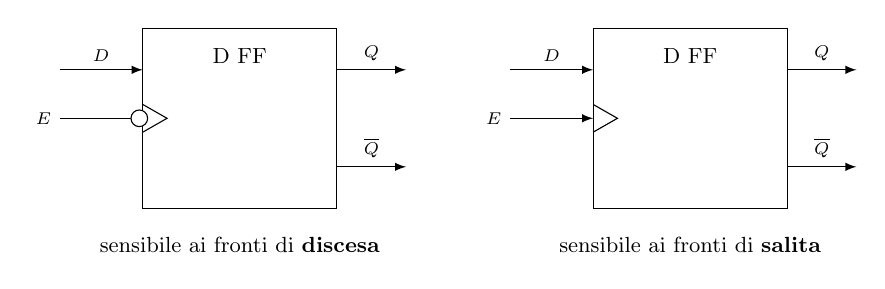
\begin{tikzpicture}[scale=0.88, every node/.style={scale=0.88}]
%----- fronte di discesa (E falling) -----
\draw (0,0) rectangle (2.8,2.6);
\node[font=\small] at (1.4,2.2) {D FF};
\draw[-latex](-1.2,2.0)--(0,2.0) node[midway,above,font=\scriptsize]{$D$};
% clock con triangolo (fronte attivo) e piccolo cerchio (fronte di discesa)
\draw[-latex](-1.2,1.3)--(0,1.3);
\draw (0,1.1) -- (0.35,1.3) -- (0,1.5);   % triangolo sul bordo del box
\draw[fill=white] (-0.05,1.3) circle (0.12); % cerchio = fronte di discesa
\node[left, font=\scriptsize] at (-1.2,1.3) {$E$};
\draw[-latex](2.8,2.0)--(3.8,2.0) node[midway,above,font=\scriptsize]{$Q$};
\draw[-latex](2.8,0.6)--(3.8,0.6) node[midway,above,font=\scriptsize]{$\overline{Q}$};
\node[below, font=\small] at (1.4,-0.3) {sensibile ai fronti di \textbf{discesa}};

%----- fronte di salita (E rising) -----
\begin{scope}[xshift=6.5cm]
\draw (0,0) rectangle (2.8,2.6);
\node[font=\small] at (1.4,2.2) {D FF};
\draw[-latex](-1.2,2.0)--(0,2.0) node[midway,above,font=\scriptsize]{$D$};
\draw[-latex](-1.2,1.3)--(0,1.3);
\draw (0,1.1) -- (0.35,1.3) -- (0,1.5);   % triangolo = fronte di salita
\node[left, font=\scriptsize] at (-1.2,1.3) {$E$};
\draw[-latex](2.8,2.0)--(3.8,2.0) node[midway,above,font=\scriptsize]{$Q$};
\draw[-latex](2.8,0.6)--(3.8,0.6) node[midway,above,font=\scriptsize]{$\overline{Q}$};
\node[below, font=\small] at (1.4,-0.3) {sensibile ai fronti di \textbf{salita}};
\end{scope}
\end{tikzpicture}
\end{center}

\medskip
\noindent\textcolor{teal}{\textbf{Cosa succede se togliamo l'invertitore (NOT)?}}\\
Senza l'inverter, sia il master che lo slave riceverebbero lo stesso segnale $E$ contemporaneamente, vanificando tutto:
\begin{itemize}[leftmargin=1.5em,itemsep=2pt]
  \item Quando $E=1$, entrambi i Latch diventerebbero trasparenti nello stesso istante. Il segnale $D$ fluirebbe senza ostacoli attraverso il master, passerebbe per $P$ e attraverserebbe immediatamente lo slave arrivando a $Q$. L'intero circuito agirebbe come un banale Latch D trasparente, perdendo del tutto la preziosa sensibilità al fronte.
  \item Quando $E=0$, entrambi i Latch si chiuderebbero e isolerebbero simultaneamente.
\end{itemize}
L'inverter è quindi il vero \emph{segreto} del sistema: garantendo che i due Latch non siano \textbf{mai trasparenti contemporaneamente}, li forza a passarsi il dato come in una staffetta, permettendo al segnale di raggiungere l'uscita solo nell'esatto istante della commutazione.

% ======================================================================
% Pagina 7 (13/04/2026)
% ======================================================================

\section{Tecnica trigger-edge}

La \textbf{tecnica trigger-edge} (sensibile al fronte) rappresenta l'architettura standard per i moderni Flip-Flop integrati. Al posto dell'approccio master-slave (due latch in cascata), questa tecnica usa \textbf{sei porte} NOR (o NAND) organizzate in \textbf{tre latch SR}: due latch di ingresso ($G_1$--$G_2$ e $G_3$--$G_4$) generano i comandi $R$ ed $S$ per il latch di uscita ($G_5$--$G_6$). Nello schema, con porte NOR, il flip-flop è sensibile al \textbf{fronte di discesa} del clock.

\begin{fitcenter}
\begin{circuitikz}[line width=0.6pt]
\node[nor port] (G1) at (0, 4.0) {};
\node[nor port] (G2) at (0, 2.6) {};
\node[nor port, number inputs=3] (G3) at (0, 1.2) {};
\node[nor port] (G4) at (0,-0.2) {};
\node[nor port] (G5) at (4.0, 2.4) {};
\node[nor port] (G6) at (4.0, 1.0) {};
\foreach \g in {1,...,6}{ \node[font=\scriptsize] at ($(G\g.west)!0.5!(G\g.out)+(0.05,0)$) {$G_\g$}; }
% G1 -> G2
\draw (G1.out) -| (0.5,3.3) -| (-1.5,0 |- G2.in 1) -- (G2.in 1);
% G2 -> G1, G3, G5 (comando R del latch di uscita)
\coordinate (n2) at (0.9,2.6);
\draw (G2.out) -- (n2);
\node[circle, fill, inner sep=1.1pt] at (n2) {};
\draw (n2) |- (-1.9,5.0) |- (G1.in 1);
\draw (n2) |- (-1.5,1.9) |- (G3.in 1);
\draw (n2) -- (2.5,2.6) |- (G5.in 1);
\node[above, font=\scriptsize] at (1.7,2.6) {$R$};
% G3 -> G4, G6 (comando S del latch di uscita)
\coordinate (n3) at (0.5,1.2);
\draw (G3.out) -- (n3);
\node[circle, fill, inner sep=1.1pt] at (n3) {};
\draw (n3) |- (-1.5,0.5) |- (G4.in 1);
\draw (n3) -- (2.2,1.2) |- (G6.in 2);
\node[above, font=\scriptsize] at (1.4,1.2) {$S$};
% G4 -> G1, G3
\draw (G4.out) -| (1.3,-1.1) -| (-3.1,0 |- G1.in 2) -- (G1.in 2);
\node[circle, fill, inner sep=1.1pt] at (-3.1,0 |- G3.in 3) {};
\draw (-3.1,0 |- G3.in 3) -- (G3.in 3);
% clock
\draw (G2.in 2) -- (-2.3,0 |- G2.in 2) -- (-2.3,0 |- G3.in 2) -- (G3.in 2);
\node[jump crossing] (JC) at (-3.1,1.9) {};
\draw (-4.0,1.9) node[left]{CLK} -- (JC.west);
\draw (JC.east) -- (-2.3,1.9) node[circle, fill, inner sep=1.1pt] {};
% dato
\draw (G4.in 2) -- (-2.7,0 |- G4.in 2) node[above right, inner sep=1pt] {$D$};
% latch di uscita
\draw (G5.out) -- ++(0.4,0) coordinate (q) -- ++(1.0,0) node[right]{$Q$};
\draw (G6.out) -- ++(0.4,0) coordinate (qb) -- ++(1.0,0) node[right]{$\overline{Q}$};
\node[circle, fill, inner sep=1.1pt] at (q) {};
\node[circle, fill, inner sep=1.1pt] at (qb) {};
\draw (q) -- ($(G6.in 1)+(-0.4,0)$) -- (G6.in 1);
\draw (qb) -- ($(G5.in 2)+(-0.4,0)$) -- (G5.in 2);
\end{circuitikz}
\end{fitcenter}

\noindent Le porte calcolano: $G_1=\overline{G_2+G_4}$, $G_2=\overline{G_1+\text{CLK}}$,
$G_3=\overline{G_2+\text{CLK}+G_4}$, $G_4=\overline{G_3+D}$, e il latch di uscita
$Q=\overline{R+\overline{Q}}$, $\overline{Q}=\overline{S+Q}$ con $R=G_2$, $S=G_3$.
Il segreto di questo circuito sta nell'\textbf{autobloccaggio} delle porte:
\begin{itemize}[leftmargin=1.5em,itemsep=2pt]
  \item \textbf{CLK $=1$}: $G_2$ e $G_3$ sono forzate a 0, quindi $R=S=0$ e il latch di
        uscita mantiene lo stato. Intanto i latch di ingresso seguono il dato:
        $G_4=\overline{D}$ e $G_1=D$.
  \item \textbf{Fronte di discesa (CLK $1\to 0$)}: $G_2=\overline{G_1}=\overline{D}$ e
        $G_3=\overline{G_2+G_4}=D$. Se $D=1$ si ha $S=1$, $R=0$ e quindi $Q=1$; se $D=0$ si ha
        $R=1$, $S=0$ e quindi $Q=0$. In entrambi i casi $Q$ prende il valore di $D$ e
        $\overline{Q}$ quello di $\overline{D}$.
  \item \textbf{CLK $=0$ a regime}: i latch di ingresso restano bloccati. Se è stato
        catturato $D=1$, l'uscita $G_3=1$ forza $G_4=0$ qualunque sia $D$; se è stato
        catturato $D=0$, l'uscita $G_2=1$ forza $G_1=0$ e $G_3=0$. Se $D$ cambia mentre il
        clock è a regime, l'uscita resta costante.
  \item Quando il clock torna a 1, $R$ e $S$ tornano a 0 e l'uscita continua a mantenere
        il dato.
\end{itemize}
Con porte NAND si ottiene la stessa struttura (è quella dell'integrato 7474), sensibile però
al fronte di salita.

\noindent\textit{Riferimento laboratorio}: pag.\ 9–10–11–12 di
\texttt{digitale/lab3-09-2026o410-latchFF.pdf}.

% ======================================================================
\section{Ingressi sincroni e asincroni}
\label{sec:sincroni_asincroni}

\textit{(13/04/2026)}

In un sistema sequenziale pratico, è quasi sempre necessario poter forzare un dispositivo in uno stato noto (es. azzerarlo all'accensione del sistema) senza dover aspettare il battito del clock. Per questo motivo, molti Flip-Flop integrano due tipologie di ingressi contemporaneamente:

\begin{important}
\begin{itemize}[leftmargin=1.5em,itemsep=4pt]
  \item \textbf{Ingressi SINCRONI (es. Data $D$, Clock $C$):} obbediscono rigidamente alla tempistica del circuito. Un ingresso sincrono ($D$) viene letto ed applicato alle uscite \emph{esclusivamente} durante il fronte attivo del clock.
  \item \textbf{Ingressi ASINCRONI (es. Preset/Set, Clear/Reset):} agiscono come \textbf{comandi di emergenza} o priorità assoluta. Appena vengono attivati, scavalcano totalmente la logica sincrona forzando le uscite istantaneamente, a prescindere da cosa stiano facendo il clock e l'ingresso $D$.
\end{itemize}
\end{important}

\noindent Esempio di un Flip-Flop D commerciale con ingressi misti (tipico delle logiche TTL):

\begin{center}
\begin{circuitikz}[scale=0.88, every node/.style={scale=0.88}]
\draw (0,0) rectangle (2.8,3.0);
\node[font=\small] at (1.4,2.7) {FF-D};

% D sincrono
\draw[-latex](-1.4,2.4)--(0,2.4) node[midway,above,font=\scriptsize]{$D$};
% clock con triangolo
\draw[-latex](-1.4,1.5)--(0,1.5) node[midway,above,font=\scriptsize]{$C$};
\draw (0,1.3)--(0.3,1.5)--(0,1.7);   % triangolo fronte
% S asincrono
\draw[-latex](-1.4,0.6)--(0,0.6) node[midway,above,font=\scriptsize]{$S$};
% R asincrono (in basso fuori dal box principale)
\draw[-latex](1.4,-0.5)--(1.4,0) node[midway,right,font=\scriptsize]{$R$};

% Uscite
\draw[-latex](2.8,2.2)--(3.8,2.2) node[midway,above,font=\scriptsize]{$Q$};
\draw[-latex](2.8,0.8)--(3.8,0.8) node[midway,above,font=\scriptsize]{$\overline{Q}$};

\node[below=0.5cm, font=\small] at (1.4,-0.9) {FF-D con ingressi misti};
\end{circuitikz}
\end{center}

In questo simbolo, $D$ viene campionato solo sul fronte di $C$, mentre l'attivazione di $S$ (Set) o $R$ (Reset) forzerà immediatamente l'uscita indipendentemente dal clock.

% ======================================================================
\section{JK Flip-Flop}
\label{sec:jk_ff}
% ======================================================================

Il Flip-Flop (o Latch) RS originale ha un grave difetto: lo stato $R=1, S=1$ è proibito, poiché forza le uscite in uno stato incoerente. Il Flip-Flop di tipo D risolve il problema unendo gli ingressi tramite un invertitore, ma così facendo sacrifica la flessibilità di poter comandare il Set e il Reset in modo indipendente.

Il \textbf{Flip-Flop JK} risolve il problema alla radice, mantenendo due ingressi separati ($J$ per il Set e $K$ per il Reset) e introducendo un \textbf{incrocio (feedback) dalle uscite verso gli ingressi}. Questo si ottiene anteponendo due porte AND al nucleo RS centrale.

\medskip
\noindent\textbf{Il principio dell'auto-disabilitazione.}
Il trucco logico del Flip-Flop JK sta nell'usare le uscite stesse per "spegnere" i comandi ridondanti:
\begin{itemize}[leftmargin=1.5em]
    \item Se il circuito si trova nello stato $Q=1$ (e quindi $\overline{Q}=0$), il segnale $\overline{Q}$ viene retroazionato sulla porta AND dell'ingresso $J$ (Set). Essendo a $0$, disabilita completamente l'ingresso $J$. Il circuito sa di essere già a $1$, quindi ignora ulteriori richieste di Set. Allo stesso tempo, l'uscita $Q=1$ abilita la porta AND dell'ingresso $K$ (Reset).
    \item Se il circuito è nello stato $Q=0$ (e $\overline{Q}=1$), accade l'opposto: viene abilitato l'ingresso $J$ (Set) e viene disabilitato l'ingresso $K$ (Reset).
\end{itemize}
Grazie a questa intelligenza intrinseca, se applichiamo la combinazione massima $J=1, K=1$, il sistema lascerà passare \emph{solo} il comando opposto allo stato in cui si trova, trasformando la vecchia condizione "proibita" in una utilissima funzione di commutazione (Toggle).

\begin{center}
\begin{circuitikz}[scale=0.9, every node/.style={scale=0.9}]
% Central SR Flip-Flop block
\draw (0, -1.2) rectangle (2.4, 1.2);
\node[font=\large] at (0.4, 0.7) {$S$};
\node[font=\large] at (0.4, -0.7) {$R$};
\node[font=\large] at (2.0, 0.7) {$Q$};
\node[font=\large] at (2.0, -0.7) {$\overline{Q}$};

% Clock triangle on the SR block
\draw (0, -0.2) -- (0.3, 0) -- (0, 0.2);

% AND gates
\node[and port] (AJ) at (-1.5, 0.7) {};
\node[and port] (AK) at (-1.5, -0.7) {};

% Connections AND -> SR
\draw (AJ.out) -- (0, 0.7);
\draw (AK.out) -- (0, -0.7);

% CLK input (center)
\draw (-2.8, 0) node[left, font=\large] {CLK} -- (0, 0);

% Inputs J and K (aligned with CLK)
\draw (AJ.in 2) -- (AJ.in 2 -| -2.8, 0) node[left, font=\large] {$J$};
\draw (AK.in 1) -- (AK.in 1 -| -2.8, 0) node[left, font=\large] {$K$};

% Outputs and feedbacks
\draw (2.4, 0.7) -- (4.2, 0.7); % Q output line
\node[circle, fill, inner sep=1.2pt] at (3.8, 0.7) {};
% Feedback from Q to AK.in 2 (bottom loop, routed outside J/K/CLK)
\draw (3.8, 0.7) -- (3.8, -2.2) -- (-3.8, -2.2) |- (AK.in 2);

\draw (2.4, -0.7) -- (4.2, -0.7); % Qbar output line
\node[circle, fill, inner sep=1.2pt] at (3.2, -0.7) {};
% Feedback from Qbar to AJ.in 1 (top loop, routed outside J/K/CLK)
\draw (3.2, -0.7) -- (3.2, 2.2) -- (-3.8, 2.2) |- (AJ.in 1);

\node[below=0.6cm, font=\small] at (1.2,-2.8) {JK Flip-Flop};
\end{circuitikz}
\end{center}

\medskip
\noindent\textbf{Ricavo della Funzione Caratteristica.}
Dal circuito logico osserviamo che gli ingressi interni del nucleo RS diventano:
\[ S = J \cdot \overline{Q}_n \qquad \text{e} \qquad R = K \cdot Q_n \]
Partendo dall'equazione caratteristica del Flip-Flop RS, ovvero $Q_{n+1} = S + \overline{R}Q_n$, possiamo sostituire queste due espressioni:
\begin{align*}
Q_{n+1} &= (J \overline{Q}_n) + \overline{(K Q_n)} Q_n \\
        &= J \overline{Q}_n + (\overline{K} + \overline{Q}_n) Q_n \quad \text{[applicando il Teorema di De Morgan]}\\
        &= J \overline{Q}_n + \overline{K} Q_n + \underbrace{\overline{Q}_n Q_n}_{=0} \quad \text{[espandendo e applicando l'annullamento]}
\end{align*}
\noindent Otteniamo così la \textbf{Funzione caratteristica del Flip-Flop JK}:
\[
\boxed{Q_{n+1} = J\overline{Q}_n + \overline{K}Q_n}
\]

\medskip
\noindent\textcolor{teal}{\textbf{Tabella di verità e sintesi del comportamento:}}
\begin{itemize}[leftmargin=1.5em,itemsep=4pt]
  \item \textbf{$J = 0, K = 0$ (HOLD / MEMORIA):} Entrambe le porte AND d'ingresso sono bloccate (zero in uscita). Il nucleo centrale riceve la combinazione $S=0, R=0$ e quindi \textbf{mantiene in memoria} lo stato precedente ($Q_{n+1}=Q_n$).
  \item \textbf{$J = 1, K = 0$ (SET):} L'ingresso $J$ è attivo. Se il flip-flop era a $0$, viene portato a $1$. Se era già a $1$, vi rimane ($Q_{n+1}=1$).
  \item \textbf{$J = 0, K = 1$ (RESET):} L'ingresso $K$ è attivo. L'uscita viene forzatamente portata a $0$, o vi rimane se lo era già ($Q_{n+1}=0$).
  \item \textbf{$J = 1, K = 1$ (TOGGLE / COMMUTAZIONE):} Il vero punto di forza del JK. Essendo la combinazione proibita ormai innocua, l'applicazione simultanea di due '1' logici forza il sistema a \textbf{invertire il proprio stato} ad ogni fronte di clock ($Q_{n+1}=\overline{Q}_n$).
\end{itemize}
\newpage
% ======================================================================
\subsection{Esempio pratico: il Registro come "filtro anti-glitch"}
% ======================================================================

Per comprendere l'utilità pratica dei circuiti sequenziali, analizziamo un classico problema dei \textbf{circuiti combinatori}: la generazione di \emph{glitch} (stati transitori spuri). Immaginiamo di voler pilotare un \textbf{display a 7 segmenti} partendo da un dato in codice Gray (\cref{ch:gray-ascii}), utilizzando un \textbf{convertitore Gray-Binario}.

Consideriamo una transizione critica, come il passaggio dal valore 15 al valore 0:
\begin{itemize}[leftmargin=1.5em,itemsep=2pt]
    \item L'ingresso in codice Gray passa da \texttt{1000} (15) a \texttt{0000} (0). Come previsto dalla codifica Gray, commuta \textbf{un solo bit}.
    \item L'uscita in codice Binario, invece, deve passare da \texttt{1111} a \texttt{0000}: ben \textbf{4 bit devono commutare simultaneamente}.
\end{itemize}

\textbf{Il problema: i ritardi di propagazione (Glitch)}\\
Il convertitore è realizzato tramite porte logiche in cascata (tipicamente porte XOR). Poiché ogni porta possiede un proprio \textbf{ritardo fisico di propagazione}, i 4 bit in uscita non commuteranno mai nell'esatto medesimo istante. I segnali attraversano percorsi logici di lunghezza diversa, accumulando ritardi differenti.

Di conseguenza, anziché avere un salto netto $\texttt{1111} \to \texttt{0000}$, le uscite attraversano una serie caotica di stati intermedi (ad esempio, $\texttt{1111} \to \texttt{0111} \to \texttt{0011} \to \texttt{0000}$). Se il display fosse collegato direttamente all'uscita del convertitore, l'osservatore vedrebbe una rapida e fastidiosa sequenza di numeri errati (sfarfallio) prima della stabilizzazione sul valore corretto. Questi stati transitori indesiderati prendono il nome di \emph{glitch}.

\begin{center}
\begin{tikzpicture}[
    >=latex,
    font=\small,
    box/.style={
        draw=black!70, 
        thick, 
        minimum width=2.6cm, 
        minimum height=1.4cm, 
        align=center, 
        rounded corners=2pt
    },
    highlight_box/.style={
        box, 
        fill=teal!10, 
        draw=teal!80
    }
]

% Blocchi
\node[box] (conv) {CONVERTITORE\\[0.5ex] \scriptsize Gray $\to$ Binario};
\node[highlight_box, right=2.5cm of conv] (reg) {\textbf{REGISTRO}\\[0.5ex] \scriptsize (Banco D Flip-Flop)};
\node[box, right=2.5cm of reg] (disp) {DISPLAY\\[0.5ex] \scriptsize 7 segmenti};

% Collegamenti dati
\draw[->, thick] (conv) -- (reg) node[midway, above] {\scriptsize Dati "sporchi"};
\draw[->, thick] (reg) -- (disp) node[midway, above] {\scriptsize Dati "puliti"};

% Input / Output (frecce esterne per far capire il flusso)
\draw[<-, thick] (conv.west) -- ++(-1.8,0) node[midway, above, font=\scriptsize, color=gray!80!black] {Codice Gray (In)};
\draw[->, thick] (disp.east) -- ++(1.8,0) node[midway, above, font=\scriptsize, color=gray!80!black] {Valore visivo (Out)};

% Segnale di CLOCK (freccia che entra dal basso nel registro)
\draw[->, thick, teal] (reg.south) ++(0,-1.2) -- (reg.south) 
    node[at start, below] {\textbf{Segnale di CLOCK}};

\end{tikzpicture}
\end{center}

\textbf{La soluzione: il Registro come barriera di temporizzazione}\\
Per risolvere il problema alla radice, si interpone un \textbf{Registro} (un banco di Flip-Flop di tipo D in parallelo, comandati da un unico clock) tra il circuito combinatorio e il display. Il registro agisce come una "fotocamera" sincronizzata, mascherando i transienti:

\begin{enumerate}[leftmargin=1.5em,itemsep=2pt]
    \item \textbf{Fase di assestamento (Glitch):} Mentre il convertitore ricalcola il dato, generando gli stati spuri, il segnale di Clock è mantenuto a riposo. I Flip-Flop ignorano i cambiamenti in ingresso, e il display continua a mostrare stabilmente il numero precedente (15).
    \item \textbf{Stato stazionario:} Si attende un tempo sufficiente affinché tutte le porte del convertitore abbiano finito di commutare. Ora l'uscita è un \texttt{0000} stabile e definitivo.
    \item \textbf{Campionamento (Fronte attivo):} Proprio in questo istante di stabilità ("acque calme"), si invia un fronte di salita al Clock del registro. I Flip-Flop catturano simultaneamente il nuovo dato pulito e lo trasferiscono al display in blocco.
\end{enumerate}

\noindent La traccia seguente, acquisita con un analizzatore logico (Digilent Analog Discovery 2), mostra l'efficacia di questa tecnica:
\begin{center}
  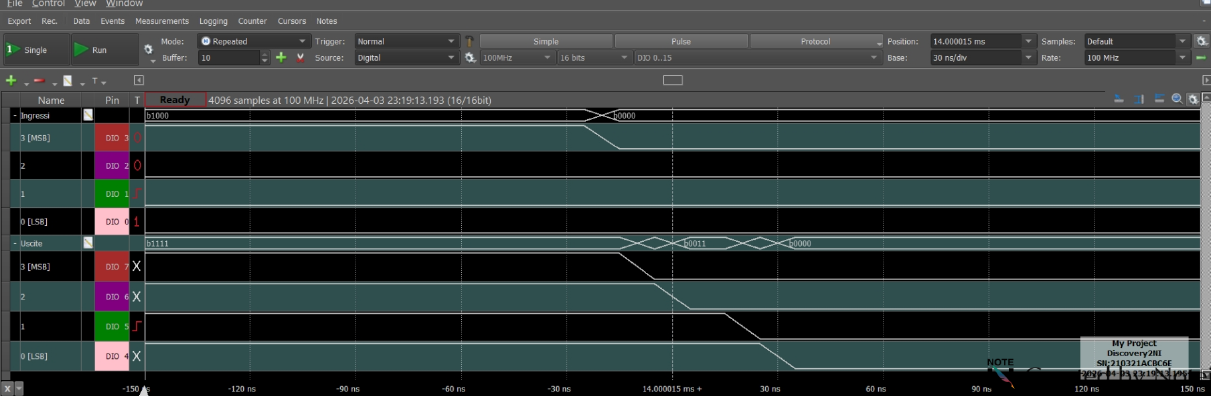
\includegraphics[width=1\linewidth]{1.png}
\end{center}

\noindent Osservando il transitorio (a cavallo di $t=14{,}000015\,\text{ms}$), è evidente come le singole linee in uscita dal blocco combinatorio scendano a zero in istanti sfalsati, generando temporaneamente un dato spuro (es. \texttt{b0011}). 
Grazie all'azione di campionamento del registro, tali irregolarità vengono confinate a monte: il circuito a valle viene aggiornato con precisione chirurgica e perfetta sincronia solo in corrispondenza del fronte di clock, garantendo un'uscita netta e priva di sfarfallii.

% ======================================================================
\section*{Riepilogo del Capitolo}

\begin{important}
La logica sequenziale introduce la memoria tramite retroazione: un anello di porte incrociate (\textbf{Latch SR}) conserva un bit, e l'evoluzione verso \textbf{Latch D} e \textbf{Flip-Flop JK} elimina lo stato proibito e separa nettamente la sensibilità al \emph{livello} (Latch) dalla sensibilità al \emph{fronte} (Flip-Flop).
\end{important}

\begin{note}
\textbf{Formule fondamentali (funzioni caratteristiche):}
\begin{itemize}
    \item \textbf{Latch RS (NOR):} $Q(t+\Delta t) = S + \overline{R}\,Q(t)$; stato proibito $R=S=1$.
    \item \textbf{Latch RS con Enable:} $Q(t+\Delta t) = ES + \overline{RE}\,Q(t)$ ($E=0$ hold, $E=1$ trasparente).
    \item \textbf{Latch D:} $Q(t+\Delta t) = DE + \overline{E}\,Q(t)$ (vincolo $R=\overline{D}$, $S=D$: elimina lo stato proibito).
    \item \textbf{Flip-Flop JK:} $Q_{n+1} = J\overline{Q}_n + \overline{K}Q_n$ ($J=K=1 \Rightarrow$ toggle, $Q_{n+1}=\overline{Q}_n$).
    \item \textbf{Sensibilità al fronte:} ottenuta con tecnica Master-Slave o trigger-edge (due o tre latch pilotati in controfase/autobloccaggio).
\end{itemize}
\end{note}

